\documentclass[11pt]{article}
\usepackage{theme}
\usepackage{shortcuts}
\usepackage{graphicx}
\usepackage{stmaryrd}
\usepackage{amsmath}
\usepackage{amsfonts}
% Document parameters
% Document title
\title{Assignment 1 (ML for TS) - MVA 2023/2024}
\author{
Louis-Marie Lovichi \email{lm.lovichi@me.com} \\ % student 1
Gaspard Berthelier \email{gaspard.berthelier@student-cs.fr} % student 2
}

\begin{document}
\maketitle

\section{Introduction}

\paragraph{Objective.} This assignment has three parts: questions about the convolutional dictionary learning, the spectral features and a data study using the DTW. 

\paragraph{Warning and advice.} 
\begin{itemize}
    \item Use code from the tutorials as well as from other sources. Do not code yourself well-known procedures (e.g. cross validation or k-means), use an existing implementation. 
    \item The associated notebook contains some hints and several helper functions.
    \item Be concise. Answers are not expected to be longer than a few sentences (omitting calculations).
\end{itemize}



\paragraph{Instructions.}
\begin{itemize}
    \item Fill in your names and emails at the top of the document.
    \item Hand in your report (one per pair of students) by Tuesday 7\textsuperscript{th} November 23:59 PM.
    \item Rename your report and notebook as follows:\\ \texttt{FirstnameLastname1\_FirstnameLastname2.pdf} and\\ \texttt{FirstnameLastname1\_FirstnameLastname2.ipynb}.\\
    For instance, \texttt{LaurentOudre\_CharlesTruong.pdf}.
    \item Upload your report (PDF file) and notebook (IPYNB file) using this link: \footnotesize{\href{https://docs.google.com/forms/d/e/1FAIpQLSdTwJEyc6QIoYTknjk12kJMtcKllFvPlWLk5LbyugW0YO7K6Q/viewform?usp=sf_link}{docs.google.com/forms/d/e/1FAIpQLSdTwJEyc6QIoYTknjk12kJMtcKllFvPlWLk5LbyugW0YO7K6Q/viewform?usp=sf\_link}}.
\end{itemize}


\section{Convolution dictionary learning}

\begin{exercise}
Consider the following Lasso regression:
\begin{equation}\label{eq:lasso}
    \min_{\beta\in\RR^p} \frac{1}{2}\norm{y-X\beta}^2_2 \quad + \quad \lambda \norm{\beta}_1
\end{equation}
where $y\in\RR^n$ is the response vector, $X\in\RR^{n\times p}$ the design matrix, $\beta\in\RR^p$ the vector of regressors and $\lambda>0$ the smoothing parameter.

Show that there exists $\lambda_{\max}$ such that the minimizer of~\eqref{eq:lasso} is $\mathbf{0}_p$ (a $p$-dimensional vector of zeros) for any $\lambda > \lambda_{\max}$. 
\end{exercise}

\begin{solution}  % ANSWER HERE

Notons $f(\beta,\lambda)=\frac{1}{2}||y-X\beta||^2_2+\lambda ||\beta||_1$.\\

On cherche à trouver $\lambda_{\max}$ tel que $\forall \lambda > \lambda_{\max},\, \textrm{argmin}_{\beta}f(\beta,\lambda)=0$.\\

Notons $\beta_\lambda^*=\textrm{argmin}_{\beta}f(\beta,\lambda)$. On a alors : $f(\beta^*_\lambda) \leq f(0,\lambda)=\frac{1}{2}||y||^2_2$ \\

C'est à dire :

$$\frac{1}{2}\sum_i (y_i-[X\beta_\lambda^*]_i)^2+\lambda \sum_i |\beta^*_{\lambda,i}|\leq \frac{1}{2}\sum_i y_i^2 $$

$$\Leftrightarrow \, \sum_{i,j} [X_{ij}^2\beta_{\lambda,j}^{*2}-2y_iX_{ij}\beta_{\lambda,j}^*] + 2\lambda \sum_i |\beta_{\lambda,i}^*| \leq 0$$

$$\Leftrightarrow \, \sum_{i,j} [X_{ij}^2|\beta^*_{\lambda,j}| + 2\lambda ]|\beta_{\lambda,j}^*| \leq \sum_{i,j} 2y_iX_{ij}\beta_{\lambda,j}^*$$

Donc par majoration :

$$\sum_{i,j} [X_{ij}^2|\beta^*_{\lambda,j}| + 2\lambda ]|\beta_{\lambda,j}^*| \leq \sum_{i,j} 2|y_i||X_{ij}||\beta_{\lambda,j}^*|$$

Si on fait l'hypothèse $\beta_{\lambda}^* \neq 0$ :

$$\Leftrightarrow \, \forall (i,j),\, X_{ij}^2|\beta^*_{\lambda,j}| + 2\lambda \leq 2|y_i||X_{ij}|$$
$$\Leftrightarrow \, \forall (i,j),\, 0\leq X_{ij}^2|\beta^*_{\lambda,j}| \leq 2(|y_i||X_{ij}|-\lambda)$$

On constate donc qu'il suffit de prendre $\lambda > \lambda_{\max}=\|y\|_{\infty}\|X\|_{\max}$ pour avoir une contradiction car le terme à droite serait négatif. Ainsi pour $\lambda > \lambda_{\max}$, on a bien $\beta^*_{\gamma}=0$.

\begin{equation}
    \lambda_{\max} = \|y\|_{\infty}\|X\|_{\infty}
\end{equation}

\end{solution}

\begin{exercise}
For a univariate signal $\mathbf{x}\in\mathbb{R}^n$ with $n$ samples, the convolutional dictionary learning task amounts to solving the following optimization problem:

\begin{equation}
\min_{(\mathbf{d}_k)_k, (\mathbf{z}_k)_k \\ \norm{\mathbf{d}_k}_2^2\leq 1} \quad\norm{\mathbf{x} - \sum_{k=1}^K \mathbf{z}_k * \mathbf{d}_k }^2_2 \quad + \quad\lambda \sum_{k=1}^K \norm{\mathbf{z}_k}_1
\end{equation}

where $\mathbf{d}_k\in\mathbb{R}^L$ are the $K$ dictionary atoms (patterns), $\mathbf{z}_k\in\mathbb{R}^{N-L+1}$ are activations signals, and $\lambda>0$ is the smoothing parameter.

Show that
\begin{itemize}
    \item for a fixed dictionary, the sparse coding problem is a lasso regression (explicit the response vector and the design matrix);
    \item for a fixed dictionary, there exists $\lambda_{\max}$ (which depends on the dictionary) such that the sparse codes are only 0 for any $\lambda > \lambda_{\max}$. 
\end{itemize}
\end{exercise}

\begin{solution}  % ANSWER HERE


Let's consider a fixed dictionnary $(d_k)_k$ and the sparce coding problem :

$$(z_{k})_k^{\lambda*} = \textrm{argmin}_{(z_k)_k}\, \|x-\sum_k z_k * d_k \|_2^2+\lambda \sum_k \|z_k\|_1$$

The quantity $z_k*d_k[n]$ can be defined for $n \in \llbracket 1,N\rrbracket$ with :

$$z_k*d_k[n] = \sum_{m=1}^{N} \tilde{z}_k[m]\tilde{d}_k[n-m]$$

where $\tilde{z_k}$ and $\tilde{d_k}$ are padded versions of $z_k$ and $d_k$, of size $N$ and with zeros if $z_k$ or $d_k$ is not defined. So:

$$z_k*d_k[n] = (\tilde{d_k^{(n)}})^T\tilde{z_k}$$

where $\tilde{d_k^{(n)}}$ is equal to $\tilde{d}_k$ with an inversion followed by n-2 circular translations of the indexes. 

We can concatenate the $\tilde{d_k}^{(n)}$ vectors as lines into a $\tilde{D_k}$ matrix of size $N*N$ such that $z_k*d_k$ is the vector $\tilde{D_k}\tilde{z}_k$ of size $N$. So we have :

$$\sum_{k=1}^K z_k*d_k = \sum_{k=1}^K \tilde{D_k}\tilde{z_k}$$

We can express this sum as one big matrix product by concatenating $\tilde{D_k}$ along the columns ($\tilde{D}$ matrix of size $N*KN$) and $\tilde{z}_k$ as one vector $\tilde{z}$ of size $NK$, which gives us :

$$\sum_{k=1}^K z_k*d_k = \tilde{D}\tilde{z} $$

As it turns out : 

$$||\tilde{z}||_1 = \sum_{k,n} |z_k[n]|=\sum_{k=1}^K \sum_n |z_k[n]| = \sum_{k=1}^K \|z_k\|_1$$

So we have reformulated the problem as :

$$(z_{k})_k^{\lambda*} = \textrm{argmin}_{(z_k)_k}\, \|x-\tilde{D}\tilde{z}\|_2^2+\lambda \|\tilde{z}\|_1$$

By factorizing by $\frac{1}{2}$ and renaming $2\lambda$ as $\lambda$, $\tilde{z}$ as $\beta$, $\tilde{D}$ as $X$ and taking $p = KN$, we have exactly the same problem as Question 1. So the sparse coding problem is indeed a lasso regression.

\begin{equation}
    \lambda_{\max} = \|x\|_{\infty}\|\tilde{D}\|_{\infty}
\end{equation}

\end{solution}

\section{Spectral feature}

Let $X_n$ ($n=0,\dots,N-1)$ be a weakly stationary random process with zero mean and autocovariance function $\gamma(\tau):= \mathbb{E}(X_n X_{n+\tau})$.
Assume the autocovariances are absolutely summable, \ie $\sum_{\tau\in\mathbb{Z}} |\gamma(\tau)| < \infty$, and square summable, \ie $\sum_{\tau\in\mathbb{Z}} \gamma^2(\tau) < \infty$.
Denote by $f_s$ the sampling frequency, meaning that the index $n$ corresponds to the time instant $n / f_s$ and for simplicity, let $N$ be even.


The \textit{power spectrum} $S$ of the stationary random process $X$ is defined as the Fourier transform of the autocovariance function:
\begin{equation}
    S(f) := \sum_{\tau=-\infty}^{+\infty}\gamma(\tau)e^{-2\pi f\tau/f_s}.
\end{equation}
The power spectrum describes the distribution of power in the frequency space. 
Intuitively, large values of $S(f)$ indicates that the signal contains a sine wave at the frequency $f$.
There are many estimation procedures to determine this important quantity, which can then be used in a machine learning pipeline.
In the following, we discuss about the large sample properties of simple estimation procedures, and the relationship between the power spectrum and the autocorrelation.

(Hint: use the many results on quadratic forms of Gaussian random variables to limit the amount of calculations.)

\begin{exercise}
    In this question, let $X_n$ ($n=0,\dots,N-1)$ be a Gaussian white noise.

    \begin{itemize}
        \item Calculate the associated autocovariance function and power spectrum. (By analogy with the light, this process is called ``white'' because of the particular form of its power spectrum.)
    \end{itemize}

\end{exercise}

\begin{solution}

    By definition of a white noise, $X=(X_n)_n$ is wide-sense stationary, centered and $\gamma_X(\tau)=\sigma^2 \delta(\tau)$ where $\sigma^2 = V(X_0)=E(X_0^2)$. 

    So the autocovariance is equal to $\sigma^2\delta(\tau)$.\\
    Now we can compute the power spectrum :

    $$S(f) = \sum_{\tau \in \mathbb{Z}} \gamma(\tau) e^{-2i\pi f\tau/f_s}=\sigma^2 \sum_{\tau \in \mathbb{Z}} \delta(\tau) e^{-2i\pi f\tau/f_s}=\sigma^2 $$

    The power spectrum is constant for all frequences and equal to the variance.

\end{solution}


\begin{exercise}

    A natural estimator for the autocorrelation function is the sample autocovariance
    \begin{equation}
        \hat{\gamma}(\tau) := (1/N) \sum_{n=0}^{N-\tau-1} X_n X_{n+\tau}
    \end{equation}
    for $\tau=0,1,\dots,N-1$ and $\hat{\gamma}(\tau):=\hat{\gamma}(-\tau)$ for $\tau=-(N-1),\dots,-1$.
    \begin{itemize}
        \item Show that $\hat{\gamma}(\tau)$ is a biased estimator of $\gamma(\tau)$ but asymptotically unbiased.
        What would be a simple way to de-bias this estimator?
    \end{itemize}

\end{exercise}

\begin{solution}

    Let's compute the bias of the sample autocovariance :
    $$E(\hat{\gamma}(\tau))=\frac{1}{N}\sum_{n=0}^{N-\tau-1}E(X_nX_{n+\tau})=\frac{1}{N}\sum_{n=0}^{N-\tau-1}\gamma(\tau)=\frac{N-\tau}{N}\gamma(\tau)$$
    $$\Rightarrow \textrm{bias} = E(\hat{\gamma}(\tau))-\gamma(\tau) = \frac{-\tau}{N} \gamma(\tau)$$
    We can see that for $\tau\neq 0$, we have bias $\neq 0$ so the estimator is biased. But the bias tends towards 0 as $N$ increases, so it is asymptotically unbiased.

    We could compute a de-biased estimator by setting $\tilde{\gamma}(\tau) = \dfrac{N}{N - \tau} \hat{\gamma}(\tau)$.

\end{solution}

\begin{exercise}
    Define the discrete Fourier transform of the random process $\{X_n\}_n$ by
    \begin{equation}
        J(f) := (1/\sqrt{N})\sum_{n=0}^{N-1} X_n e^{-2\pi\iu f n/f_s}
    \end{equation}
    The \textit{periodogram} is the collection of values $|J(f_0)|^2$, $|J(f_1)|^2$, \dots, $|J(f_{N/2})|^2$ where $f_k = f_s k/N$.
    (They can be efficiently computed using the Fast Fourier Transform.)
    \begin{itemize}
        \item Write $|J(f_k)|^2$ as a function of the sample autocovariances.
        \item For a frequency $f$, define $f^{(N)}$ the closest Fourier frequency $f_k$ to $f$.
        Show that $|J(f^{(N)})|^2$ is an asymptotically unbiased estimator of $S(f)$ for $f>0$.
    \end{itemize}
\end{exercise}

\begin{solution}


    We have :
    $$|J(f)|^2 = J(f)J(f)^* = \frac{1}{N}(\sum_{n=0}^{N-1}X_ne^{-2i\pi fn/f_s})(\sum_{m=0}^{N-1}X_ne^{+2i\pi fn/f_s})$$
    $$=\frac{1}{N}(\sum_{n=0}^{N-1} X_n^2+\sum_{0\leq n<m}^{m=N-1}X_nX_m(e^{-2i\pi f(n-m)/f_s}+e^{-2i\pi f(m-n)/f_s}))$$
    $$=\hat{\gamma}(0)+\frac{1}{N}(\sum_{n=0}^{N-1}\sum_{\tau=1}^{N-1-n}X_nX_{n+\tau}(e^{-2i\pi f\tau/f_s}+e^{2i\pi f\tau/f_s}))$$
    Let's note $h(\tau) = e^{-2i\pi f \tau/fs}$. We get :
    $$=\hat{\gamma}(0)+\sum_{\tau=1}^{N-1}(h(\tau)+h(-\tau))\frac{1}{N}(\sum_{n=0}^{N-1-\tau}X_nX_{n+\tau})$$
    $$=\hat{\gamma}(0)+\sum_{\tau=1}^{N-1}\hat{\gamma}(\tau)(h(\tau)+h(-\tau))$$
    Since $\hat{\gamma}(-\tau) = \hat{\gamma}(\tau)$ and $h(0)=1$, we obtain :
    $$|J(f)|^2 =\sum_{\tau=-(N-1)}^{N-1}\hat{\gamma}(\tau)h(\tau)$$
    So for $f=f_k=\frac{f_sk}{N}$, we get :
    $$|J(f_k)|^2 = \sum_{\tau=-(N-1)}^{N-1}\hat{\gamma}(\tau)e^{-2i\pi \tau k/N} $$
    For $f = f^{(N)}$, we get :
    $$E(|J(f^{(N)})|^2) = \sum_{\tau=-(N-1)}^{N-1}E(\hat{\gamma}(\tau))e^{-2i\pi \tau f^{(N)}/ f_s}=\sum_{\tau=-(N-1)}^{N-1}\frac{N-\tau}{N}\gamma(\tau)e^{-2i\pi \tau f^{(N)}/ f_s} $$
    We must show that this quantity tends towards $S(f)$ as $N$ increases. We have :
    $$|S(f)-E(|J(f^{(N)})|^2)| = |\sum_{\tau \in \mathbb{Z}} \gamma(\tau)e^{-2i\pi f\tau/f_s}-\sum_{\tau=-(N-1)}^{N-1} \frac{N-\tau}{N}\gamma(\tau)e^{-2i\pi \tau f^{(N)}/f_s}|  $$
    $$= |\sum_{|\tau|\geq N} \gamma(\tau)h(\tau)+\sum_{\tau=-(N-1)}^{N-1} \gamma(\tau)(e^{-2i\pi f\tau/f_s}-(1-\frac{\tau}{N})e^{-2i\pi\tau f^{(N)}/f_s})|$$
    $$\leq \sum_{|\tau|\geq N} |\gamma(\tau)|+\sum_{\tau=-(N-1)}^{N-1} |\gamma(\tau)|(|e^{-2i\pi f\tau/f_s}-e^{-2i\pi\tau f^{(N)}/f_s}|+\frac{|\tau|}{N})$$
    We have : $|e^{-2i\pi f\tau/f_s}+e^{-2i\pi\tau f^{(N)}/f_s}| = |2i\sin(i\pi\tau(f^{(N)}-f)\frac{1}{f_s})e^{-i\pi\tau(f+f^{(N)})/f_s}|$\\
    $= 2|\sin(i\pi\tau(f^{(N)}-f)\frac{1}{f_s})|\leq 2\min(1,\pi\frac{|\tau|}{f_s}|f^{(N)}-f|)$\\ \\
    By definition of $f^{(N)}$, we have $\lim_{N\rightarrow +\infty} \, |f^{(N)}-f|=0$. \\
    Also, since $\sum |\gamma(\tau)|$ is summable, we have $\lim_{N\rightarrow +\infty}\sum_{|\tau|\geq N}|\gamma(\tau)|=0$\\ \\
    For $\epsilon>0$, let's use $N_0$ such that $\forall N \geq N_0,\, \max(\sum_{|\tau|\geq N}|\gamma(\tau)|,|f^{(N)}-f|) \leq \epsilon$.
    For $N\geq N_0$:
    $$|S(f)-E(|J(f^{(N)})|^2)| \leq \epsilon + \sum_{\tau=-(N-1)}^{N-1}|\gamma(\tau)|(2\min(1,|\tau|\frac{\pi}{f_s}|f^{(N)}-f|)+\frac{|\tau|}{N}) $$
    Let's note $h(\tau,N)\rightarrow_{N\rightarrow \infty}=0$ the term inside the sum.\\
    We now have for $\tilde{N}\geq 0$:
    $$|S(f)-E(|J(f^{(N)})|^2)|\leq \epsilon + \sum_{|\tau|<\tilde{N}}h(\tau,N) + \sum_{\begin{tabular}{c}
    $\tau=-(N-1)$\\
    $|\tau|\geq \tilde{N}$
    \end{tabular}}^{N-1}h(\tau,N) $$
    The fist sum has a finite number of elements that tend towards 0. We can easily choose $\tilde{N}\geq N_0$ such that $\forall N \geq \tilde{N}$ :
    $$|S(f)-E(|J(f^{(N)})|^2)|\leq 2\epsilon + \sum_{\tilde{N}\leq |\tau|\leq N-1}h(\tau,N) $$
    Where inside the sum :
    $$h(\tau,N) \leq |\gamma(\tau)|[\,2\min(1,\epsilon \frac{\pi}{f_s})+1] $$
    By taking $\epsilon$ small enough we get inside the sum : $h(\tau,N)\leq (1+\epsilon 2\pi /f_s)|\gamma(\tau)|$
    By summability of $|\gamma(\tau)|$ once again, the sum above tends to 0 hence we have proven that the estimator is asymptotically unbiased.    

\end{solution}

\begin{exercise}\label{ex:wn-exp}
    In this question, let $X_n$ ($n=0,\dots,N-1)$ be a Gaussian white noise with variance $\sigma^2=1$ and set the sampling frequency to $f_s=1$ Hz
    \begin{itemize}
        \item For $N \in \{200, 500, 1000\}$, compute the \textit{sample autocovariances} ($\hat{\gamma}(\tau)$ vs $\tau$) for 100 simulations of $X$.
        Plot the average value as well as the average $\pm$ the standard deviation.
        What do you observe?
        \item For $N \in \{200, 500, 1000\}$, compute the \textit{periodogram} ($|J(f_k)|^2$ vs $f_k$) for 100 simulations of $X$.
        Plot the average value as well as the average $\pm$ the standard deviation.
        What do you observe?
    \end{itemize}
    Add your plots to Figure~\ref{fig:wn-exp}.
    
\begin{figure}
    \centering
    \begin{minipage}[t]{0.3\textwidth}
    \centerline{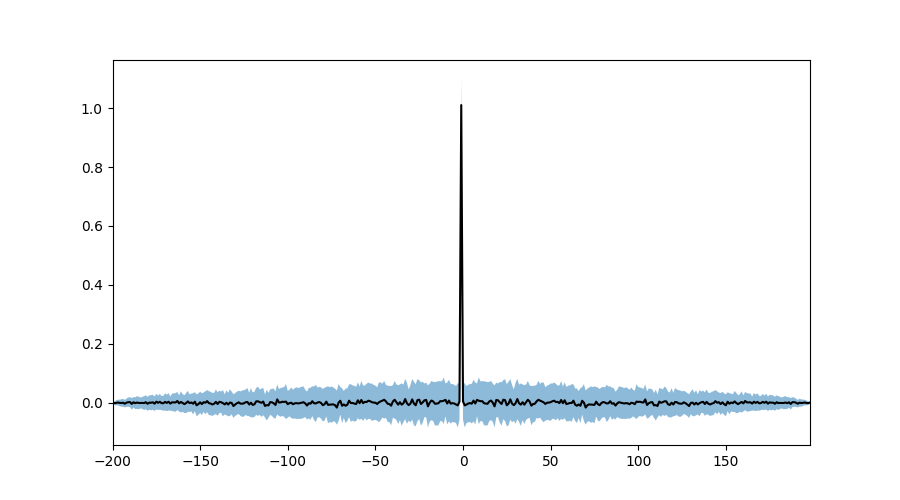
\includegraphics[width=\textwidth]{imgs/autocov200.png}}
    \centerline{Autocovariance ($N=200$)}
    \end{minipage}
    \begin{minipage}[t]{0.3\textwidth}
    \centerline{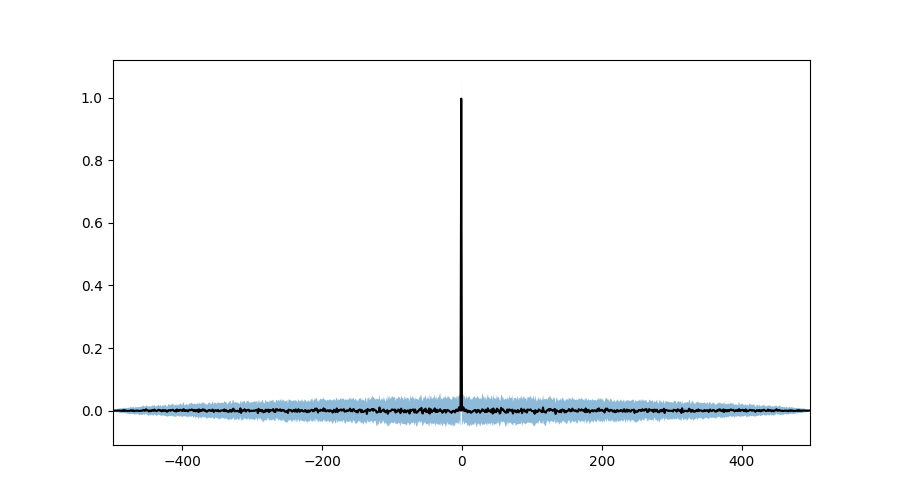
\includegraphics[width=\textwidth]{imgs/autocov500.png}}
    \centerline{Autocovariance ($N=500$)}
    \end{minipage}
    \begin{minipage}[t]{0.3\textwidth}
    \centerline{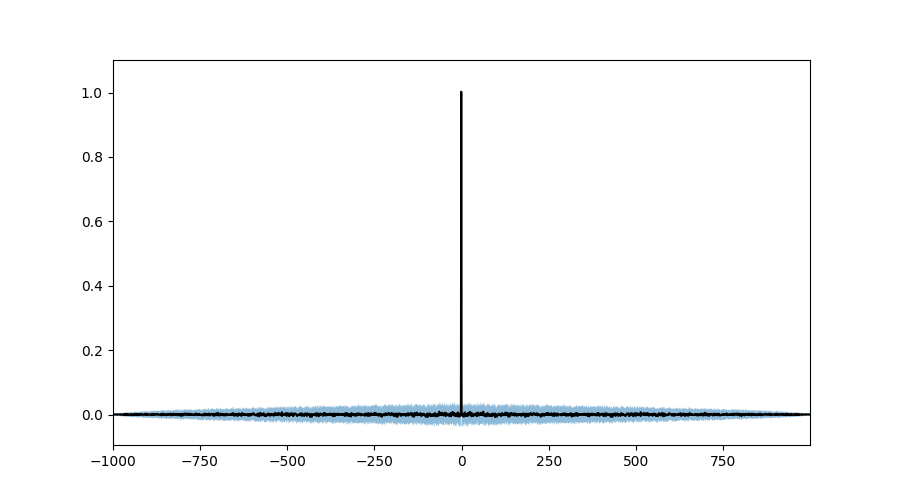
\includegraphics[width=\textwidth]{imgs/autocov1000.png}}
    \centerline{Autocovariance ($N=1000$)}
    \end{minipage}
    \vskip1em
    \begin{minipage}[t]{0.3\textwidth}
    \centerline{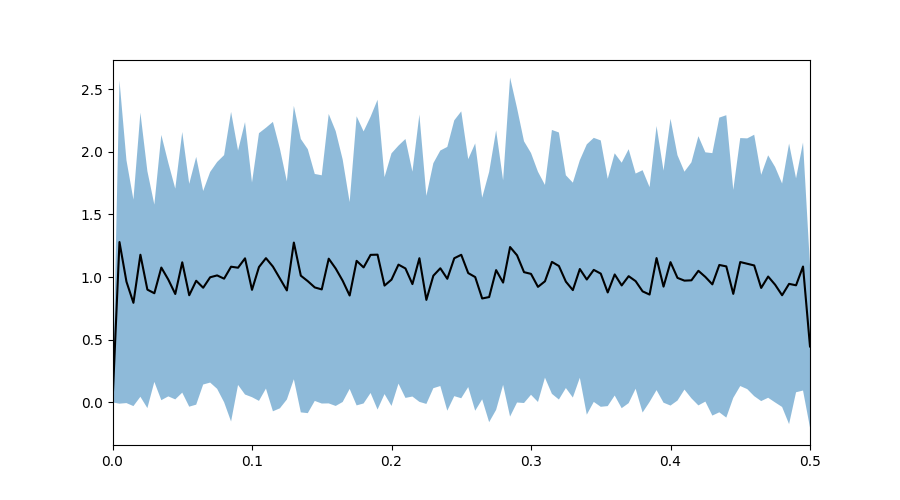
\includegraphics[width=\textwidth]{imgs/periodo200.png}}
    \centerline{Periodogram ($N=200$)}
    \end{minipage}
    \begin{minipage}[t]{0.3\textwidth}
    \centerline{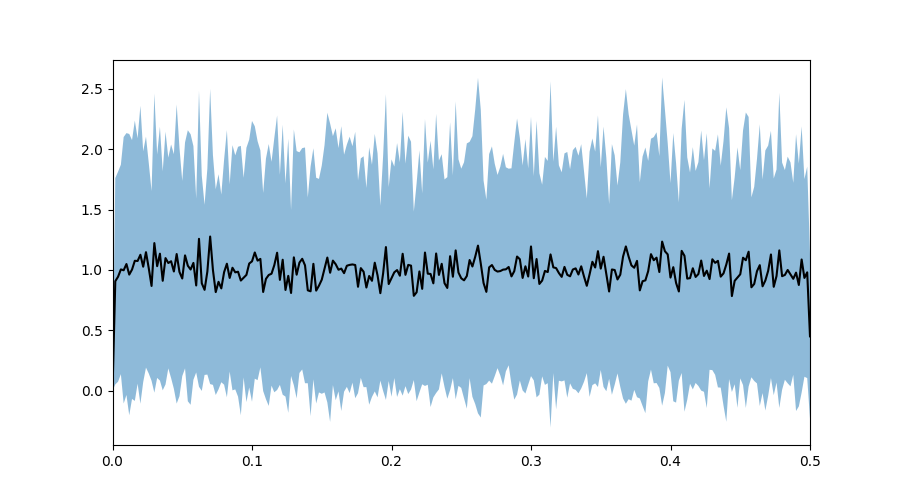
\includegraphics[width=\textwidth]{imgs/periodo500.png}}
    \centerline{Periodogram ($N=500$)}
    \end{minipage}
    \begin{minipage}[t]{0.3\textwidth}
    \centerline{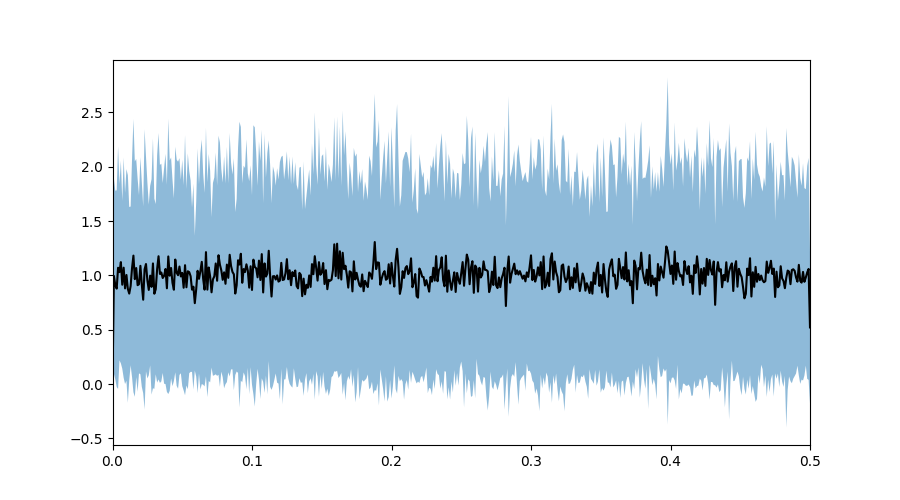
\includegraphics[width=\textwidth]{imgs/periodo1000.png}}
    \centerline{Periodogram ($N=1000$)}
    \end{minipage}
    \vskip1em
    \caption{Autocovariances and periodograms of a Gaussian white noise (see Question~\ref{ex:wn-exp}).}
    \label{fig:wn-exp}
\end{figure}

\end{exercise}

\begin{solution}
    
    \begin{itemize}
        \item We can conclude that the variance of the estimator for the autocovariance decreases as $N \rightarrow + \infty$.
        \item We can conclude that the variance of the estimator for the periodogram does not decrease as $N \rightarrow + \infty$.
    \end{itemize}

\end{solution}

\begin{exercise}
    We want to show that the estimator $\hat{\gamma}(\tau)$ is consistent, \ie it converges in probability when the number $N$ of samples grows to $\infty$ to the true value ${\gamma}(\tau)$.
    In this question, assume that $X$ is a wide-sense stationary \textit{Gaussian} process.
    \begin{itemize}
        \item Show that for $\tau>0$ 
    \begin{equation}
       \text{var}(\hat{\gamma}(\tau)) = (1/N) \sum_{n=-(N-\tau-1)}^{n=N-\tau-1} \left(1 - \frac{\tau + |n|}{N}\right) \left[\gamma^2(n) + \gamma(n-\tau)\gamma(n+\tau)\right].
    \end{equation}
    (Hint: if $\{Y_1, Y_2, Y_3, Y_4\}$ are four centered jointly Gaussian variables, then $\mathbb{E}[Y_1 Y_2 Y_3 Y_4] = \mathbb{E}[Y_1 Y_2]\mathbb{E}[Y_3 Y_4] + \mathbb{E}[Y_1 Y_3]\mathbb{E}[Y_2 Y_4] + \mathbb{E}[Y_1 Y_4]\mathbb{E}[Y_2 Y_3]$.) 
    \item Conclude that $\hat{\gamma}(\tau)$ is consistent.
    \end{itemize}
\end{exercise}

\begin{solution}

    \begin{itemize}
        \item For $\tau >0$ :
        $$V(\hat{\gamma}(\tau))=\frac{1}{N^2}V(\sum_{n=0}^{N-\tau-1} X_nX_{n+\tau})=\frac{1}{N^2}\sum_{0\leq n\leq m\leq N-L-1} (2-\delta_{n,m})\textrm{cov}(X_nX_{n+\tau},X_mX_{m+\tau})$$
    
        With $2-\delta_{n,m}=1$ if $n=m$, otherwise 2. Also :
    
        $$\textrm{cov}(X_nX_{n+\tau},X_mX_{m+\tau}) = E(X_nX_{n+\tau}X_mX_{m+\tau})-E(X_nX_{n+\tau})E(X_mX_{m+\tau})$$
    
        It is not indicated that the $X_n$ variables are centered but judging by the hint given in the subject, we will assume they are :
    
        $$\textrm{cov}(X_nX_{n+\tau},X_mX_{m+\tau})=E(X_nX_m)E(X_{n+\tau}X_{m+\tau})+E(X_nX_{m+\tau})E(X_{n+\tau}X_m)$$
    
        $$=r_X(n,m)r_X(n+\tau,m+\tau)+r_X(n,m+\tau)r_X(n+\tau,m) $$
    
        Also, we can rewrite the double sum as follows : 
    
        $$\sum_{0\leq n\leq m\leq N-L-1} (2-\delta_{n,m})\textrm{cov}(X_nX_{n+\tau},X_mX_{m+\tau}) = \sum_{n=0}^{N-L-1}\sum_{k=0}^{N-L-1-n}(2-\delta_k) \textrm{cov}(X_nX_{n+\tau},X_{n+k}X_{n+k+\tau}) $$
    
        $$=\sum_{n=0}^{N-L-1}\sum_{k=0}^{N-L-1-n}(2-\delta_k)[r_X(n,n+k)r_X(n+\tau,n+\tau+k)+r_X(n,n+\tau+k)r_X(n+\tau,n+k)] $$
    
        $$=\sum_{n=0}^{N-L-1}\sum_{k=0}^{N-L-1-n} (2-\delta_k)[\gamma(k)^2+\gamma(\tau+k)\gamma(\tau-k)]$$
    
        The switch from the correlation coefficients to the intercorrelation coefficients with no dependency on $n$ comes from the stationary hypothesis. So we have :
    
        $$V(\hat{\gamma}(\tau)) = \frac{1}{N^2} \sum_{k=0}^{N-L-1}\sum_{n=0}^{N-L-1-k}(2-\delta_k)[\gamma(k)^2+\gamma(\tau+k)\gamma(\tau-k)]$$
    
        Let's call $h(k) = \gamma(k)^2+\gamma(\tau+k)\gamma(\tau-k)$. It does not depend on $n$. So :
    
        $$V(\hat{\gamma}(\tau)) = \frac{1}{N}\sum_{n=0}^{N-L-1}(1-\frac{L+n}{N})(2-\delta_n)h(n) $$
        $$V(\hat{\gamma}(\tau)) = \frac{1}{N}\sum_{n=0}^{N-L-1}(1-\frac{L+n}{N})(2-\delta_n)h(n) $$
    
        Since $h(-n)=h(n)$, we actually get :
    
        $$ V(\hat{\gamma}(\tau)) = \frac{1}{N}\sum_{n=-(N-L-1)}^{N-L-1}(1-\frac{L+|n|}{N})h(n)$$

        \item So, the Byenaymé-Tcheybychev inequality let us write : 

        $$\mathbb{P}(|\hat{\gamma}(\tau) - \gamma(\tau)| > t) \leq \dfrac{\mathbb{V}(\hat{\gamma}(\tau))}{t^2} \underset{n \rightarrow + \infty}{\rightarrow} 0$$
    
        Thus, $\hat{\gamma}(\tau)$ is consistent.
        
    \end{itemize}

\end{solution}

Contrary to the correlogram, the periodogram is not consistent.
It is one of the most well-known estimators that is asymptotically unbiased but not consistent.
In the following question, this is proven for a Gaussian white noise but this holds for more general stationary processes.
\begin{exercise}
    Assume that $X$ is a Gaussian white noise (variance $\sigma^2$) and let $A(f):=\sum_{n=0}^{N-1} X_n \cos(-2\pi f n/f_s$ and $B(f):=\sum_{n=0}^{N-1} X_n \sin(-2\pi f n/f_s$.
    Observe that $J(f) = (1/N) (A(f) + \iu B(f))$.
    \begin{itemize}
        \item Derive the mean and variance of $A(f)$ and $B(f)$ for $f=f_0, f_1,\dots, f_{N/2}$ where $f_k=f_s k/N$.
        \item What is the distribution of the periodogram values $|J(f_0)|^2$, $|J(f_1)|^2$, \dots, $|J(f_{N/2})|^2$.
        \item What is the variance of the $|J(f_k)|^2$? Conclude that the periodogram is not consistent.
        \item Explain the erratic behavior of the periodogram in Question~\ref{ex:wn-exp} by looking at the covariance between the $|J(f_k)|^2$.
    \end{itemize}
    
\end{exercise}

\begin{solution}

    \begin{itemize}
        \item Since $\mathbb{E}(X_n) = 0$, on a $\mathbb{E}[A(f)] = \mathbb{E}[B(f)] = 0$. For $f = f_s \dfrac{k}{N}$, we compute : 
        
        \begin{align*}
            \mathbb{V}(A(f)) & = \sum_{n=0}^{N-1} cos^2(-2\pi k \dfrac{n}{N})\mathbb{V}(X_n)\\
            & = \dfrac{\sigma^2}{2} \sum_{n=0}^{N-1} (cos(-4\pi k \dfrac{n}{N}) + 1 ) \\
            & = N\dfrac{\sigma^2}{2}
        \end{align*}

        Similarly, we compute : 

        \begin{align*}
            \mathbb{V}(B(f)) & = N\dfrac{\sigma^2}{2}
        \end{align*}

        \item We obtain $|J(f_k)|^2 = \dfrac{1}{N} (A(f_k)^2 + B(f_k)^2)$.
        $|J(f_k)|^2$ is the sum of two independant Gaussian with mean equals $0$ and variance $N\dfrac{\sigma^2}{2}$, then, $|J(f_k)|^2$ follows $\dfrac{\sigma^2}{2} \chi^2(2)$, where $\chi_2(2)$ is a chi-square distribution with 2 degrees of freedom.

        \item Then, $\mathbb{V}(|J(f_k)|^2) = \sigma^4$ and we conclude that the periodogram is not consistent.
        
        %\item More precisely,
    \end{itemize}
    
\end{solution}

\begin{exercise}\label{q:barlett}
    As seen in the previous question, the problem with the periodogram is the fact that its variance does not decrease with the sample size.
    A simple procedure to obtain a consistent estimate is to divide the signal in $K$ sections of equal durations, compute a periodogram on each section and average them.
    Provided the sections are independent, this has the effect of dividing the variance by $K$. 
    This procedure is known as Bartlett's procedure.
    \begin{itemize}
        \item Rerun the experiment of Question~\ref{ex:wn-exp}, but replace the periodogram by Barlett's estimate (set $K=5$). What do you observe.
    \end{itemize}
    Add your plots to Figure~\ref{fig:barlett}.
\end{exercise}

\begin{solution}

\begin{itemize}
    \item We can conclude that the variance indeed decreased by a $\sqrt{5}$-factor as it is expected.
\end{itemize}

\begin{figure}
    \centering
    \begin{minipage}[t]{0.3\textwidth}
    \centerline{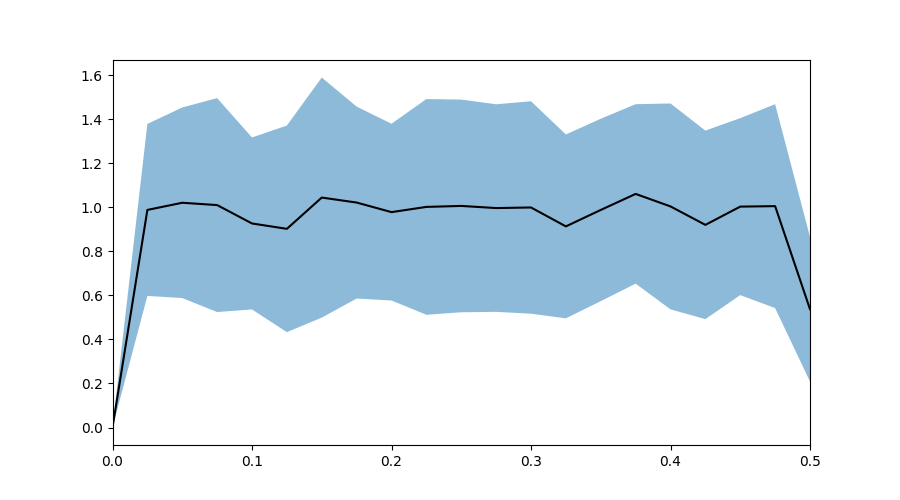
\includegraphics[width=\textwidth]{imgs/periodoK200.png}}
    \centerline{Periodogram ($N=200$)}
    \end{minipage}
    \begin{minipage}[t]{0.3\textwidth}
    \centerline{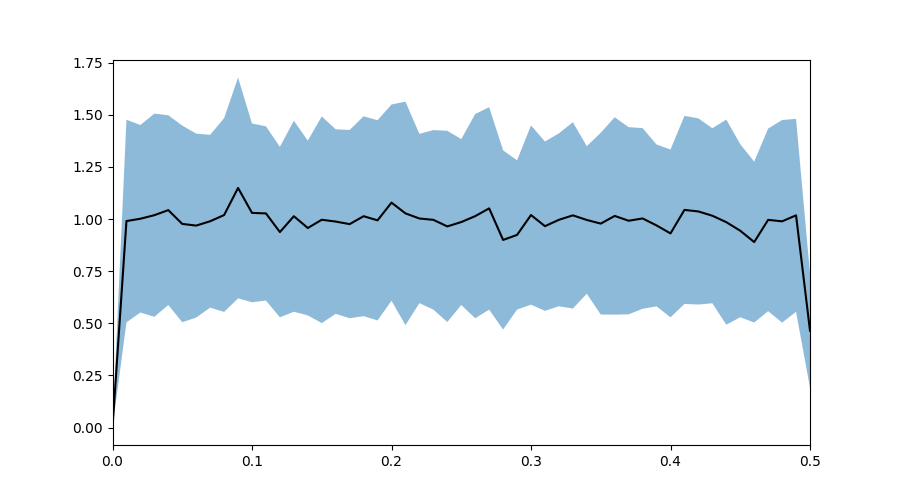
\includegraphics[width=\textwidth]{imgs/periodoK500.png}}
    \centerline{Periodogram ($N=500$)}
    \end{minipage}
    \begin{minipage}[t]{0.3\textwidth}
    \centerline{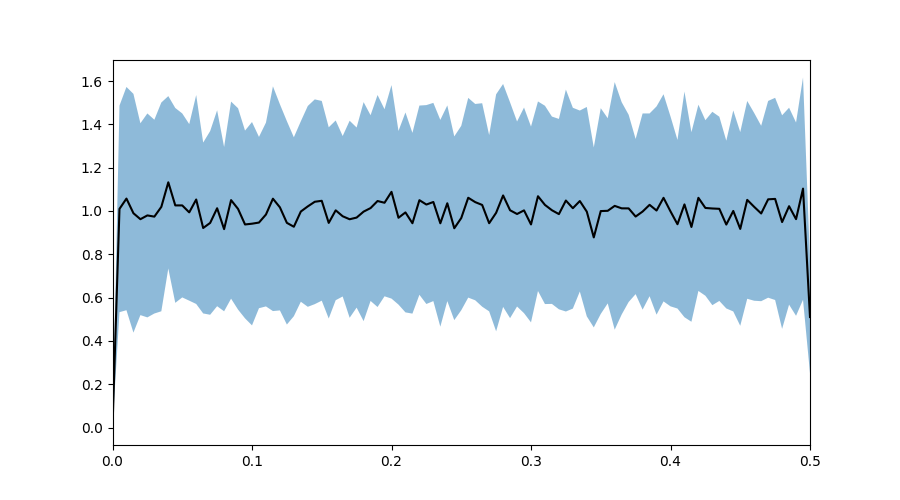
\includegraphics[width=\textwidth]{imgs/periodoK1000.png}}
    \centerline{Periodogram ($N=1000$)}
    \end{minipage}
    \vskip1em
    \caption{Barlett's periodograms of a Gaussian white noise (see Question~\ref{q:barlett}).}
    \label{fig:barlett}
\end{figure}

\end{solution}
\section{Data study}

\subsection{General information}

\paragraph{Context.}
The study of human gait is a central problem in medical research with far-reaching consequences in the public health domain. This complex mechanism can be altered by a wide range of pathologies (such as Parkinson's disease, arthritis, stroke,\ldots), often resulting in a significant loss of autonomy and an increased risk of fall. Understanding the influence of such medical disorders on a subject's gait would greatly facilitate early detection and prevention of those possibly harmful situations. To address these issues, clinical and bio-mechanical researchers have worked to objectively quantify gait characteristics.

Among the gait features that have proved their relevance in a medical context, several are linked to the notion of step (step duration, variation in step length, etc.), which can be seen as the core atom of the locomotion process. Many algorithms have therefore been developed to automatically (or semi-automatically) detect gait events (such as heel-strikes, heel-off, etc.) from accelerometer and gyrometer signals.

\paragraph{Data.}
Data are described in the associated notebook.

\subsection{Step classification with the dynamic time warping (DTW) distance}

\paragraph{Task.} The objective is to classify footsteps then walk signals between healthy and non-healthy.

\paragraph{Performance metric.} The performance of this binary classification task is measured by the F-score.


\begin{exercise}
Combine the DTW and a k-neighbors classifier to classify each step. Find the optimal number of neighbors with 5-fold cross-validation and report the optimal number of neighbors and the associated F-score. Comment briefly.
\end{exercise}

\begin{solution}

With 5-fold cross-validation, we can conclude that the optimal number of neighbors is 3 whose associated F1-score is $0.786$. You can find the code in the notebook. We have randomly shuffle the train et test datasets to ensure good F1-score (the initial train et test datasets did not provide such a F1-score).

    \begin{figure}
        \centering
        \centerline{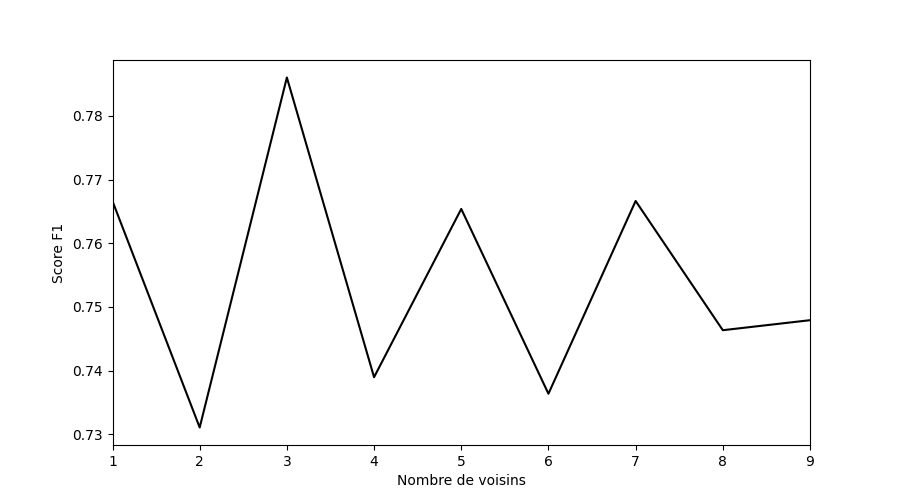
\includegraphics[width=\textwidth]{imgs/kselection.png}}
        \vskip1em
        \caption{Selection of the optimal number of neighbors $k$ via the associated F-score.}
        \label{fig:kselection}
    \end{figure}

\end{solution}

\newpage
\begin{exercise}\label{q:class-errors}
Display on Figure~\ref{fig:class-errors} a badly classified step from each class (healthy/non-healthy).
\end{exercise}

\begin{solution}
\begin{figure}
    \centering
    \begin{minipage}[t]{\textwidth}
    \centerline{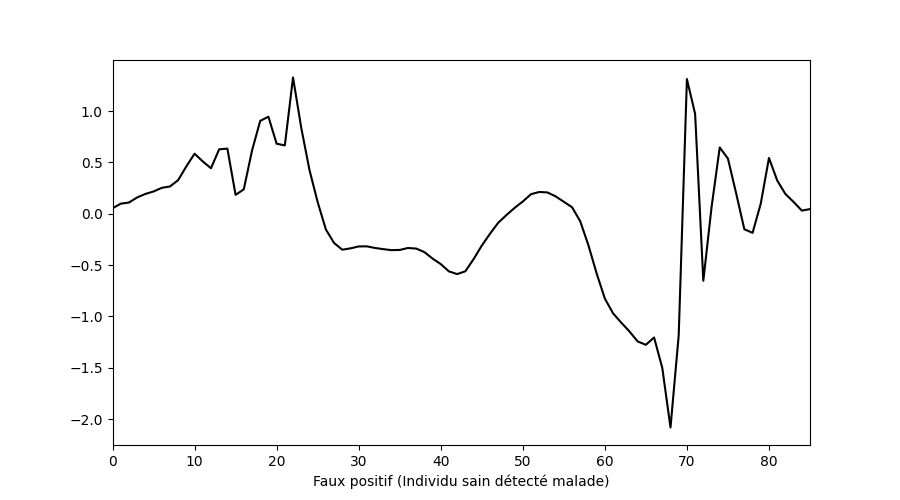
\includegraphics[width=0.9\textwidth]{imgs/FP.png}}
    \centerline{Badly classified healthy step}
    \end{minipage}
    \vskip1em
    \begin{minipage}[t]{\textwidth}
    \centerline{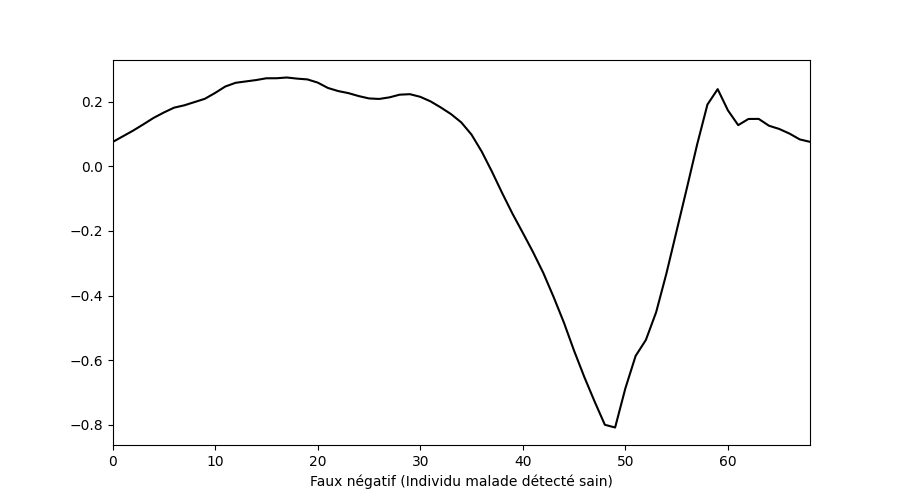
\includegraphics[width=0.9\textwidth]{imgs/FN.png}}
    \centerline{Badly classified non-healthy step}
    \end{minipage}
    \vskip1em
    \caption{Examples of badly classified steps (see Question~\ref{q:class-errors}).}
    \label{fig:class-errors}
\end{figure}
\end{solution}


\end{document}
